\newpage
\subsection{Thêm món vào giỏ, đặt món, phê duyệt đơn hàng}
\subsubsection{Diagram}
\begin{figure}[!h]
    \begin{center}
        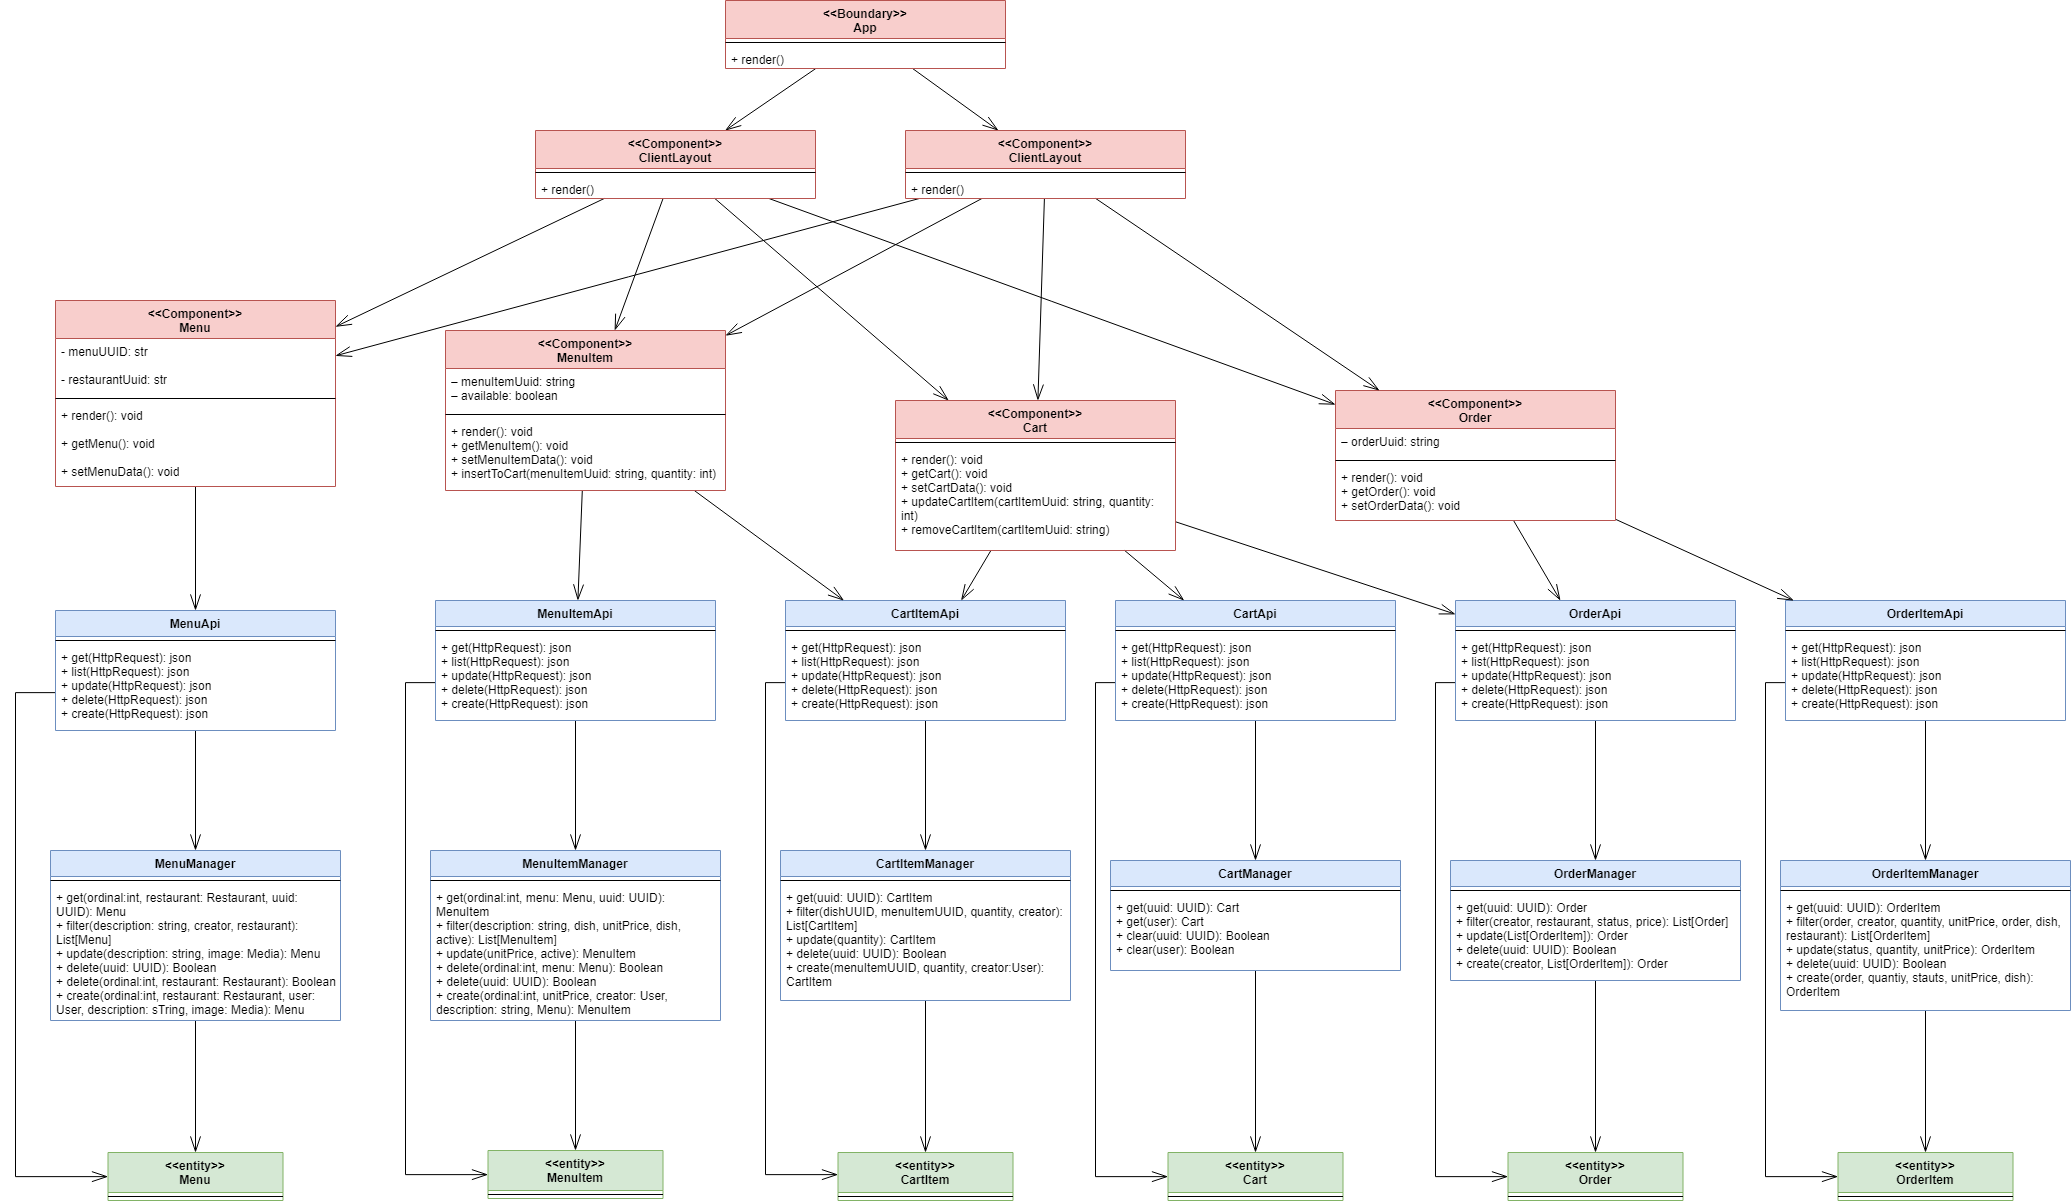
\includegraphics[scale=0.25,angle=90]{Images/ClassDiagram/order.png}
    \end{center}
    \hspace{0.3cm}
    \caption{entity class diagram}
\end{figure}
\newpage
\subsubsection{Mô tả diagram}
\subsubsubsection{class \textbf{ClientLayout}}
\begin{itemize}
    \item \textbf{Chức năng}: quản lý các component xuất hiện trong giao diện khách hàng.
    \item \textbf{Attributte} :
    \item \textbf{Methods}:
    \begin{itemize}
        \item render(): void
    \end{itemize}
\end{itemize}
\subsubsubsection{class \textbf{StaffLayout}}
\begin{itemize}
    \item \textbf{Chức năng}: quản lý các component xuất hiện trong giao diện nhân viên nhà hàng.
    \item \textbf{Attributte} :
    \item \textbf{Methods}:
    \begin{itemize}
        \item render(): void
    \end{itemize}
\end{itemize}
\subsubsubsection{class \textbf{Menu}}
\begin{itemize}
    \item \textbf{Chức năng}: Hiển thị menu của một nhà hàng.
    \item \textbf{Attributte} :
    \begin{itemize}
        \item restaurantUuid: string
    \end{itemize}
    \item \textbf{Methods}:
    \begin{itemize}
        \item[+] render(): void
        \item[+] getMenu(): void
        \item[+] setMenuData(): void
    \end{itemize}
\end{itemize}
\subsubsubsection{class \textbf{MenuItem}}
\begin{itemize}
    \item \textbf{Chức năng}: Hiển thị chi tiết một menu item của một nhà hàng.
    \item \textbf{Attributte} :
    \begin{itemize}
        \item menuItemUuid: string
        \item available: boolean
    \end{itemize}
    \item \textbf{Methods}:
    \begin{itemize}
        \item[+] render(): void
        \item[+] getMenuItem(): void
        \item[+] setMenuItemData(): void
        \item[+] insertToCart(menuItemUuid: string, quantity: int)
    \end{itemize}
\end{itemize}
\subsubsubsection{class \textbf{Cart}}
\begin{itemize}
    \item \textbf{Chức năng}: Hiển thị giỏ hàng của người dùng.
    \item \textbf{Attributte} :
    \item \textbf{Methods}:
    \begin{itemize}
        \item[+] render(): void
        \item[+] getCart(): void
        \item[+] setCartData(): void
        \item[+] updateCartItem(cartItemUuid: string, quantity: int)
        \item[+] removeCartItem(cartItemUuid: string)
    \end{itemize}
\end{itemize}
\subsubsubsection{class \textbf{Order}}
\begin{itemize}
    \item \textbf{Chức năng}: Hiển thị 1 đơn hàng của của 1 người dùng.
    \item \textbf{Attributte} :
    \begin{itemize}
        \item orderUuid: string
    \end{itemize}
    \item \textbf{Methods}:
    \begin{itemize}
        \item[+] render(): void
        \item[+] getOrder(): void
        \item[+] setOrderData(): void
    \end{itemize}
\end{itemize}
\subsubsubsection{class \textbf{MenuApi}}
\begin{itemize}
    \item \textbf{Chức năng}: Các api liên quan đến quản lý menu.
    \item \textbf{Attributte} :
    \item \textbf{Methods}:
    \begin{itemize}
        \item[+] get(HttpRequest): json
        \item[+] list(HttpRequest): json
        \item[+] update(HttpRequest): json
        \item[+] delete(HttpRequest): json
        \item[+] filter(HttpRequest): json
    \end{itemize}
\end{itemize}
\subsubsubsection{class \textbf{MenuItemApi}}
\begin{itemize}
    \item \textbf{Chức năng}: Các api liên quan đến quản lý MenuItem.
    \item \textbf{Attributte} :
    \item \textbf{Methods}:
    \begin{itemize}
        \item[+] get(HttpRequest): json
        \item[+] list(HttpRequest): json
        \item[+] update(HttpRequest): json
        \item[+] delete(HttpRequest): json
        \item[+] filter(HttpRequest): json
    \end{itemize}
\end{itemize}
\subsubsubsection{class \textbf{CartItemApi}}
\begin{itemize}
    \item \textbf{Chức năng}: Các api liên quan đến quản lý CartItem.
    \item \textbf{Attributte} :
    \item \textbf{Methods}:
    \begin{itemize}
        \item[+] get(HttpRequest): json
        \item[+] list(HttpRequest): json
        \item[+] update(HttpRequest): json
        \item[+] delete(HttpRequest): json
        \item[+] filter(HttpRequest): json
    \end{itemize}
\end{itemize}
\subsubsubsection{class \textbf{CartApi}}
\begin{itemize}
    \item \textbf{Chức năng}: Các api liên quan đến quản lý Cart.
    \item \textbf{Attributte} :
    \item \textbf{Methods}:
    \begin{itemize}
        \item[+] get(HttpRequest): json
        \item[+] list(HttpRequest): json
        \item[+] update(HttpRequest): json
        \item[+] delete(HttpRequest): json
        \item[+] create(HttpRequest): json
    \end{itemize}
\end{itemize}
\subsubsubsection{class \textbf{OrderItemApi}}
\begin{itemize}
    \item \textbf{Chức năng}: Các api liên quan đến quản lý OrderItem.
    \item \textbf{Attributte} :
    \item \textbf{Methods}:
    \begin{itemize}
        \item[+] get(HttpRequest): json
        \item[+] list(HttpRequest): json
        \item[+] update(HttpRequest): json
        \item[+] delete(HttpRequest): json
        \item[+] create(HttpRequest): json
    \end{itemize}
\end{itemize}
\subsubsubsection{class \textbf{OrderApi}}
\begin{itemize}
    \item \textbf{Chức năng}: Các api liên quan đến quản lý Order.
    \item \textbf{Attributte} :
    \item \textbf{Methods}:
    \begin{itemize}
        \item[+] get(HttpRequest): json
        \item[+] list(HttpRequest): json
        \item[+] update(HttpRequest): json
        \item[+] delete(HttpRequest): json
        \item[+] create(HttpRequest): json
    \end{itemize}
\end{itemize}
\subsubsubsection{class \textbf{MenuManager}}
\begin{itemize}
    \item \textbf{Chức năng}:  cung câp các method giúp query data từ table Menu và join các table khác nếu cần.
    \item \textbf{Attributte} :
    \item \textbf{Methods}:
    \begin{itemize}
        \item[+] get(ordinal:int, restaurant: Restaurant, uuid: UUID): Menu
        \item[+] filter(description: string, creator, restaurant): List[Menu]
        \item[+] update(description: string, image: Media): Menu
        \item[+] delete(uuid: UUID): Boolean
        \item[+] delete(ordinal:int, restaurant: Restaurant): Boolean
        \item[+] create(ordinal:int, restaurant: Restaurant, user: User, description: sTring, image: Media): Menu
    \end{itemize}
\end{itemize}
\subsubsubsection{class \textbf{MenuItemManager}}
\begin{itemize}
    \item \textbf{Chức năng}:  cung câp các method giúp query data từ table MenuItem và join các table khác nếu cần.
    \item \textbf{Attributte} :
    \item \textbf{Methods}:
    \begin{itemize}
        \item[+] get(ordinal:int, menu: Menu, uuid: UUID): MenuItem
        \item[+] filter(description: string, dish, unitPrice, dish, active): List[MenuItem]
        \item[+] update(unitPrice, active): MenuItem
        \item[+] delete(ordinal:int, menu: Menu): Boolean
        \item[+] delete(uuid: UUID): Boolean
        \item[+] create(ordinal:int, unitPrice, creator: User, description: string, Menu): MenuItem
    \end{itemize}
\end{itemize}
\subsubsubsection{class \textbf{CartItemManager}}
\begin{itemize}
    \item \textbf{Chức năng}:  cung câp các method giúp query data từ table CartItem và join các table khác nếu cần.
    \item \textbf{Attributte} :
    \item \textbf{Methods}:
    \begin{itemize}
        \item[+] get(uuid: UUID): CartItem
        \item[+] filter(dishUUID, menuItemUUID, quantity, creator): List[CartItem]
        \item[+] update(quantity): CartItem
        \item[+] delete(uuid: UUID): Boolean
        \item[+] create(menuItemUUID, quantity, creator:User): CartItem
    \end{itemize}
\end{itemize}
\subsubsubsection{class \textbf{CartManager}}
\begin{itemize}
    \item \textbf{Chức năng}:  cung câp các method giúp query data từ table Cart và join các table khác nếu cần.
    \item \textbf{Attributte} :
    \item \textbf{Methods}:
    \begin{itemize}
        \item[+] get(uuid: UUID): Cart
        \item[+] get(user): Cart
        \item[+] clear(uuid: UUID): Boolean
        \item[+] clear(user): Boolean
    \end{itemize}
\end{itemize}
\subsubsubsection{class \textbf{OrderManager}}
\begin{itemize}
    \item \textbf{Chức năng}:  cung câp các method giúp query data từ table Order và join các table khác nếu cần.
    \item \textbf{Attributte} :
    \item \textbf{Methods}:
    \begin{itemize}
        \item[+] get(uuid: UUID): Order
        \item[+] filter(creator, restaurant, status, price): List[Order]
        \item[+] update(List[OrderItem]): Order
        \item[+] delete(uuid: UUID): Boolean
        \item[+] create(creator, List[OrderItem]): Order
    \end{itemize}
\end{itemize}
\subsubsubsection{class \textbf{OrderItemManager}}
\begin{itemize}
    \item \textbf{Chức năng}:  cung câp các method giúp query data từ table OrderItem và join các table khác nếu cần.
    \item \textbf{Attributte} :
    \item \textbf{Methods}:
    \begin{itemize}
        \item[+] get(uuid: UUID): OrderItem
        \item[+] filter(order, creator, quantity, unitPrice, order, dish, restaurant): List[OrderItem]
        \item[+] update(status, quantity, unitPrice): OrderItem
        \item[+] delete(uuid: UUID): Boolean
        \item[+] create(order, quantiy, stauts, unitPrice, dish): OrderItem
    \end{itemize}
\end{itemize}